%****************************************************
%	CHAPTER 2 - Prototype Design
%****************************************************
\chapter{Prototype Design}
\label{ch:proto}
%====================================================
\section{Conventions Used}
\label{sec:proto.conventions}
The attitude conventions used for the systems' dynamic derivations in the following Chapter:\ref{ch:dynamics} are first briefly discussed here. Often these aspects are omitted or assumed to be known already. It's important to clearly and unambiguously define a standard set of framing conventions to avoid uncertainty later. Rotation matrices are included briefly but focus is on the \emph{contrast} between a rotation and transformation operation. Both \cite{spacecraftattitutdequaternions} and \cite{rigidbodylecture} provide an in depth and thorough explanation of rotation matrices and DCM attitude representation if such concepts are unfamiliar to the reader.
%====================================================
\subsection{Reference Frames Convention}
\label{subsec:proto.conventions.frames}
%====================================================
\begin{figure}[htbp]
\centering
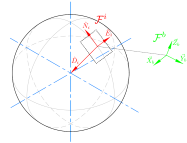
\includegraphics[width=0.6\textwidth]{figs/reference_frame}
\caption{Inertial and Body Reference Frames}
\label{fig:ref_frame}
\end{figure}
Euler (aerospace) frames are used for principle inertial and body directions (Fig:\ref{fig:ref_frame}). The inertial frame,~$\mathcal{F}^i$, is aligned such that the $\vec{X}_i$ axis is in the $\hat{N}$orth direction, $\vec{Y}_i$ is in the $\hat{E}$ast direction and $\vec{Z}_i$ is  in the $\hat{D}$ownward direction\footnote{In orbital sequences this would be toward the Earths' center. Sometimes referred to as the NED convention}. The body frame, $\mathcal{F}^b$, then has both $\vec{X}_b$ and $\vec{Y}_b$ aligned with two perpendicular arms of the quadrotors' body and the $\vec{Z}_b$ axis in the body's normal direction. The body frames' axes and their relation to the prototype design are highlighted next in Section:\ref{subsec:proto.conventions.motoraxis}. Frame superscripts $i$ and $b$ represent inertial and body frames respectively whilst vector subscripts imply the reference frame in which the vectors' coordinates exists in.
\par
The relative angular displacement between two frames is commonly measured by the three angle Euler set. The Euler set $[\phi ~\theta ~\psi]^T$ represents rotations about the $\vec{X}$,$\vec{Y}$ and $\vec{Z}$ axes respectively. Depending on how the rotation sequence is formulated, those angles can be used to construct rotation matrices which give relation to vectors or can transform coordinates. The generic equation to rotate a vector $\vec{v}$ about a (normalized) axis $\hat{n}$ by some angle $\mu$ is given by\footnote{Derived in \cite{quaddynamics}}:
\begin{equation}\label{eq:genrotationmatrix}
\vec{v}~'=\big(1-cos(\mu)\big)\big(\vec{v}\cdot \hat{n}\big)\hat{n}+cos(\mu)\vec{v}+sin(\mu)\big(\hat{n}\times\vec{v}\big)
\end{equation}
Which, when $\hat{n}$ is either $\vec{X}$,$\vec{Y}$ or $\vec{Z}$ axes, can be simplified to produce the common rotation matrices $\mathbb{R}_x(\phi)$,$\mathbb{R}_y(\theta)$ and $\mathbb{R}_z(\psi)$. Multiplication by a rotation matrix $\mathbb{R}(\cdot)$ applies a \emph{rotation} operator, the resultant vector still exists in the same reference frame, for a vector $\vec{v}\in\mathcal{F}^1$;
\begin{subequations} \label{eq:rotationoperator}
\begin{equation}\label{eq:rotationoperator.a}
\vec{v}~'=\mathbb{R}_{x}(\phi)\vec{v}
\end{equation}
\vspace{-20pt}
\begin{equation}\label{eq:rotationoperator.b}
\vec{v}~',\vec{v}\in\mathcal{F}^1
\end{equation}
\end{subequations}
\emph{\color{Gray} No subscripts are used in Eq: \ref{eq:rotationoperator} to indicate reference frame ownership because all vectors are in the same frame}
\par
A \emph{transformation} changes the vectors reference frame. The transformation is a rotation by an angle which is the difference between the resulting and principle reference frames. A transformation from frame $\mathcal{F}^1$ to $\mathcal{F}^2$ by an angle of $\phi$ about the $\vec{X}$ axis is then:
\begin{subequations}\label{eq:transformationoperator}
\begin{equation}\label{eq:transformationoperator.a}
\vec{v}_2=\mathbb{R}_x(-\phi)\vec{v}_1
\end{equation}
\vspace{-20pt}
\begin{equation}\label{eq:transformationoperator.b}
\vec{v}_2\in\mathcal{F}^2~\text{and}~\vec{v}_1\in\mathcal{F}^1
\end{equation}
\end{subequations}
The distinction between Eq:\ref{eq:rotationoperator} and Eq:\ref{eq:transformationoperator} is the sense of the angular operand, and hence the effect it has on the argument vector. The transformation of a vector from $\mathcal{F}^i$ to $\mathcal{F}^b$ is the product of three sequential operations about each of the axes. Because each subsequent rotation is applied to a new  intermediate set of axes, the sequence of those operations will effect the Euler set. Any consequences of that chosen order is something well documented in \emph{Quaternions and Rotation Sequence}, \cite{rotationsequences}. In this dissertation the ZYX sequence is used. Hence a transformation of a vector $\vec{v}$ from the inertial to the body frame is applied by:
\begin{subequations}
\begin{equation}\label{eq:inertialbodytransformation.a}
\vec{v}_b=\mathbb{R}_i^b(\psi,\theta,\phi)\vec{v}_i
\end{equation}
\vspace{-20pt}
\begin{equation}\label{eq:inertialbodytransformation.b}
\mathbb{R}_{i}^{b}\triangleq\mathbb{R}_z(-\psi)\mathbb{R}_y(-\theta)\mathbb{R}_x(-\phi)
\end{equation}
\vspace{-20pt}
\begin{equation} \label{eq:inertialbodytransformation.c}
\mathbb{R}_z(-\psi)\mathbb{R}_y(-\theta)\mathbb{R}_x(-\phi) \iff \mathbb{R}_x(\phi)\mathbb{R}_y(\theta)\mathbb{R}_z(\psi)
\end{equation}
\end{subequations}
The relation in Eq:\ref{eq:inertialbodytransformation.c} is as an inversion of the rotation matrix. A rotation matrix's inverse can be used interchangeably to maintain a positive sense of the rotational angle. To ensure clarity, for the remainder of the dissertation, a negative angular sense implies a \emph{transformation} to a different reference frame. When applicable, the order of rotation will indicate the sequence direction and the angles' sign differentiates a rotation or transformation operation.
\par
An inherent singularity does exists with such attitude representations. Indeed Quaternions are used later in Sec: \ref{subsec:dynamics.rigidbody.quaternion} in lieu of Euler angles. 3 set angular attitude representation is, however, easily understood and well suited to conventional distinctions made here. Quaternion operations are similarly sequenced in the ZYX order;
\begin{equation}
\mathbb{R}_i^b~\vec{v_i} \iff Q_z^* Q_y^* Q_x^* \otimes \vec{v_i} \otimes Q_x Q_y Q_z
\end{equation}
Wherein $\otimes$ is the Hamilton product (or quaternion operator) and $Q_i$ is a unit quaternion about some $\hat{i}$ axis. The quaternion operator and subsequent kinematics are defined later in Sec: \ref{subsec:dynamics.rigidbody.quaternion}.
%====================================================
\subsection{Motor Axis Layout}
\label{subsec:proto.conventions.motoraxis}
%====================================================

%====================================================
\section{Design}
\label{sec:proto.design}
%====================================================
\subsection{Gimbal Articulation}
\label{subsec:proto.design.actuation}
%====================================================
\subsection{Inertial Matrix Function}
\label{subsec:proto.design.inertia}
%====================================================
\subsection{Overall Aspects}
\label{subsec:proto.design.aspects}
%====================================================
\subsubsection{Vibration Damping}
%====================================================
\subsubsection{Landing Skids}
%====================================================
\subsubsection{Motors \& ESCs}
%====================================================

%====================================================
\section{System Layout}
\label{sec:proto.layout}
%====================================================
